\section{Correlation Meter}
The correlation meter monitors the stereo output of Traverso and displays the correlation coefficient of the left and the right channel signal. Unlike many other correlation meters it interprets the coefficient as a measure for stereo width and draws a gradient representing the stereo field.

In order to explain what correlation is and why it is important, we assume that a pure sine wave is played back on both the left and the right master channel. When both signals are merged (which happens if the signals are played back in mono), the resulting signal is the sum of the left and the right channel. Depending on the phase difference between the source signals, interference effects occur. That is, if two positive amplitudes are summed, the absolute value is greater, whereas if a positive and a negative amplitude are summed, the absolute value becomes smaller. In some cases this can lead to complete extinction, leaving nothing but a silent signal (\FigB\ \ref{fig_interference}).

\begin{figure}
	\centering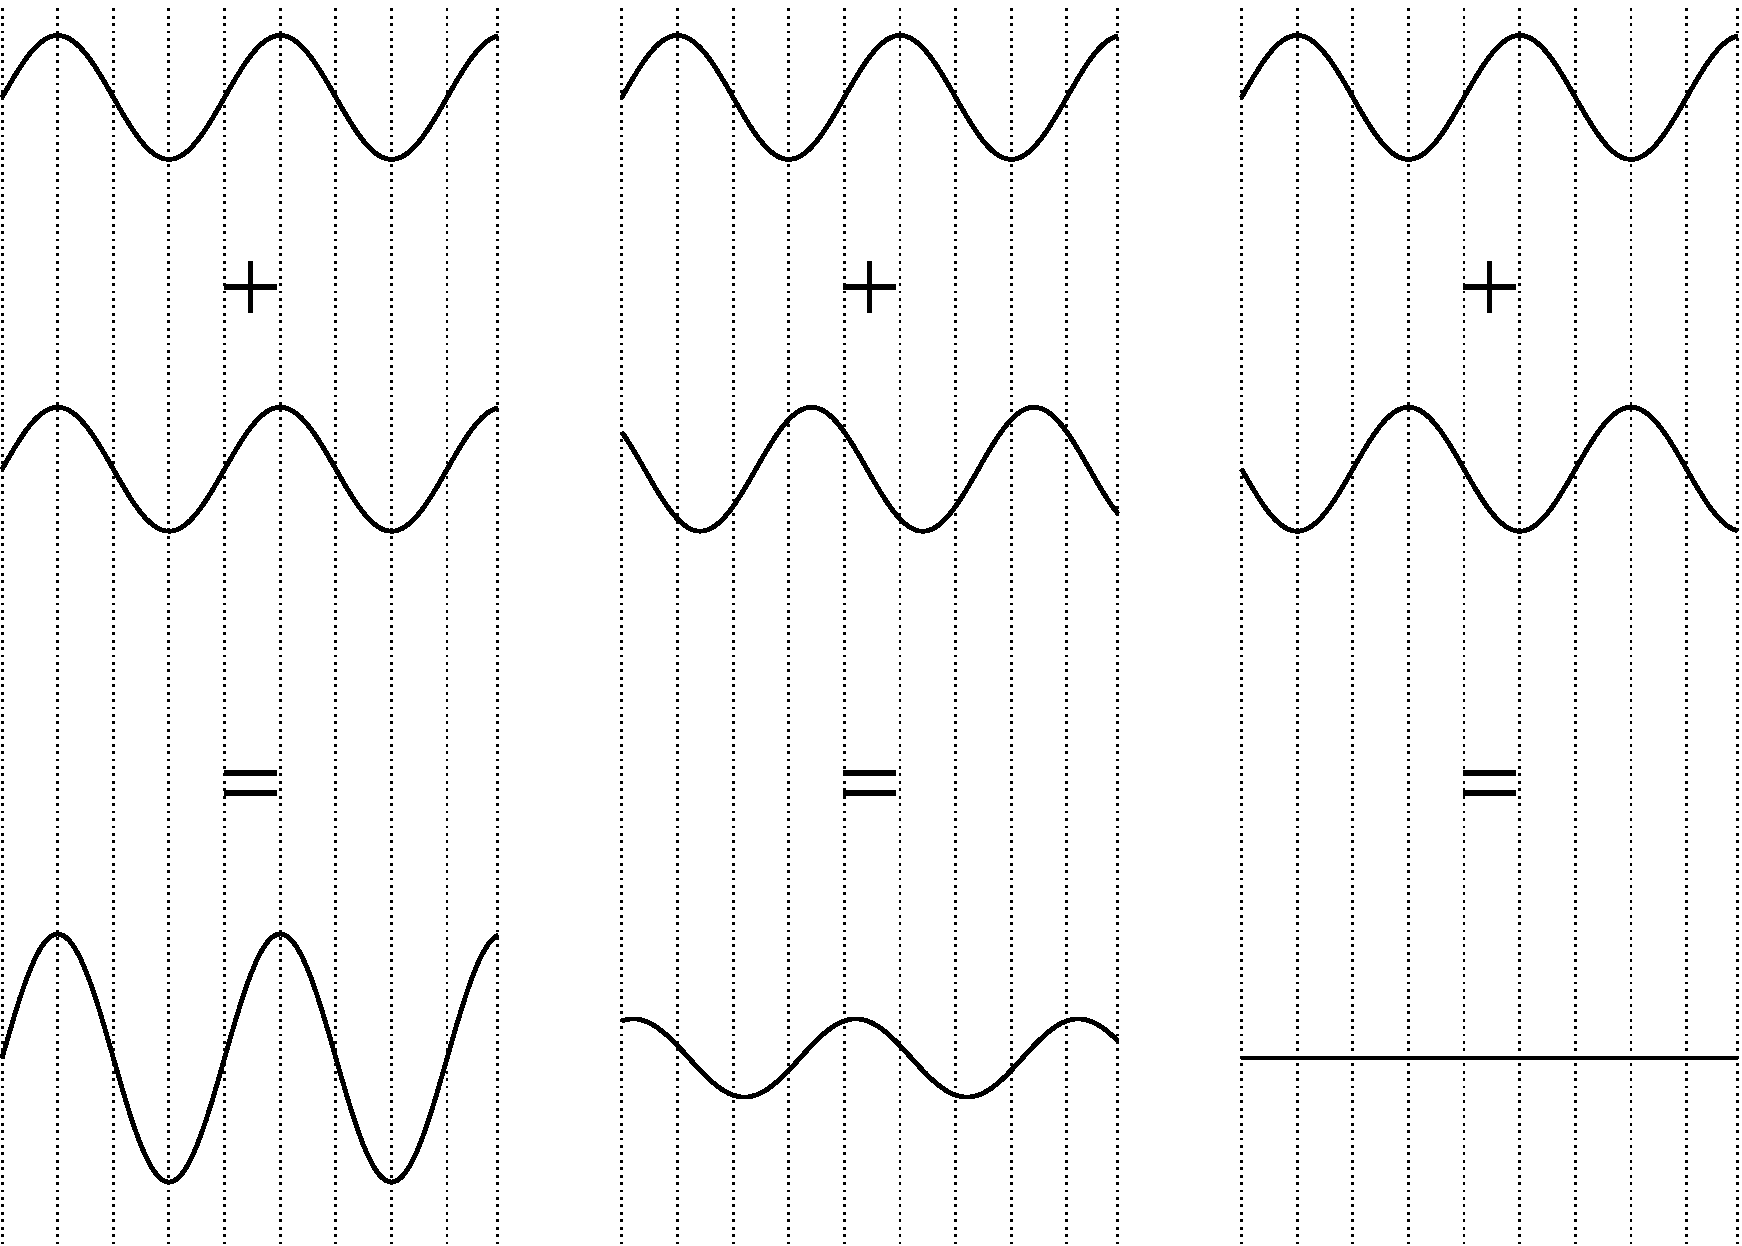
\includegraphics[width=0.8\textwidth]{images/sine01}
	\caption{When summing up two sine waves, interference can either lead to amplification (in phase, left), remain more or less unchanged (uncorrelated, middle), or lead to extinction (out of phase, right).}
	\label{fig_interference}
\end{figure}

If the two audio signals contain more complex data, e.\,g. music or spoken word, such extinction effects (also known as \emph{phase cancellations}) do not cancel out the entire signal, but merely certain frequencies, leading to a ``hollow'' or otherwise strange sound. Needless to say that such effects are rather devastating for a high quality audio production. Although it is indisputable that we should use our ears and listen to the mono signal in order to detect phase problems, computer based audio workstations allow to provide visual feedback of the audio data in many ways, which is one of the reasons for many users to prefer digital audio workstations. There are several ways to visually represent the correlation, but in order to understand how to interpret Traversos correlation meter, some more theory is required.

The amount of correlation is represented in the \emph{linear correlation coefficient} $r$, which is calculated over an array of pairs of samples $(x_i,y_i)$:
\[
r = \frac{\sum\limits_{i}(x_i - \bar{x})(y_i - \bar{y})}{\sqrt{\sum\limits_{i}(x_i - \bar{x})^2} \sqrt{\sum\limits_{i}(y_i - \bar{y})^2}}
\]
$r$ ranges from $-1.0$ to $1.0$. A value of $r = 1.0$ means the left and right signal are perfectly correlated. The master signal would be mono in that case, since there is no phase difference between the left and the right signal. The more difference there is between the two channels, the lower the correlation coefficient becomes. In case of totally uncorrelated data (which could read as ``no phase similarity whatsoever between the left and right channel''), $r$ becomes 0.0. Such a signal produces a wide stereo image with a low risk of phase cancellations when summed to mono. The difference between the signals can be further ``increased'' by one channel becoming the inverse of the other. In that case $r$ becomes $-1.0$. Negative $r$ values indicate high risk for phase cancellations.

The correlation meter of Traverso (menu ``Views $\rightarrow$ Correlation meter'') uses an intuitive way to display the correlation coefficient. Instead of focusing on the numerical value, it shows it's meaning in terms of stereo width (\FigB\ \ref{fig_cmeter01}). A gradient spreading between the left and the right speaker (marked by the L and R lines) indicates totally uncorrelated signals ($r = 0.0$) and thus a very wide stereo image. As long as the gradient does not extend beyond the L and R lines, there is no negative correlation and hence a low risk for phase cancellations. However, if it \emph{does} extend beyond the lines, phase cancellations are likely to occur if the signal is summed to mono, and the stereo image sounds unnaturally wide. This should be avoided by all means. A mono signal, on the other hand, causes the gradient to collapse to a line in the center.

\begin{figure}
	\centering
	\subfigure[Stereo, $r = 0.0$]{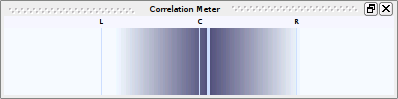
\includegraphics[width=0.7\textwidth]{images/cmeter1}}
	\subfigure[Mono, $r = 1.0$]{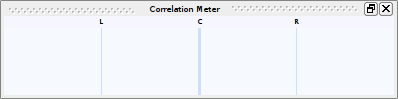
\includegraphics[width=0.7\textwidth]{images/cmeter2}}
	\subfigure[Phase cancellation, $r = -1.0$]{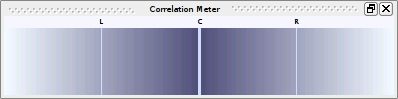
\includegraphics[width=0.7\textwidth]{images/cmeter4}}
	\caption{The correlation meter in Traverso shows the correlation coefficient of the master output signal as a gradient between two lines representing the left and the right channel. If the gradient spreads from L to R, the data is uncorrelated (correlation coefficient $r = 0.0$), and the signal has a wide stereo width (top). If the gradient is collapsed to a line, the data is perfectly correlated ($r = 1.0$), which means the signal is mono (middle). If the gradient spreads beyond the L and R lines, the correlation becomes negative, which means there's a high risk of audible phase cancellations if the output is switched to mono (bottom).}
	\label{fig_cmeter01}
\end{figure}

The correlation meter can also be used to balance the master output. If the levels of the left and right channel are well balanced, the gradient center line should ``wobble'' around the center indicator.

Since the gradient usually occupies the area between the L and R lines, the space outside of the lines is  wasted most of the time. Thus the scale of the correlation meter can be changed by pressing \sact{M}.

\section{FFT spectrum analyzer}
A spectrum analyzer using the fast fourier transformation (FFT) to calculate the spectral power distribution of an audio signal is standard equipment in digital audio workstations. The FFT spectrum analyzer in Traverso can be opened from the menu ``Views $\rightarrow$ FFT Spectrum''. It is a dock window which can either be docked into the main window, or moved freely by dragging with the mouse.

The FFT spectrum analyzer monitors the stereo output channel and decomposes the signal into frequency bands. Each band shows the highest value $dB_{left} + dB_{right}$ in its range (\FigB\ \ref{fig_fft1}). A configuration dialog can be called with \sact{E}, or from the menu opened with \sact{Q} or a right mouse button click.

\begin{figure}
	\centering
	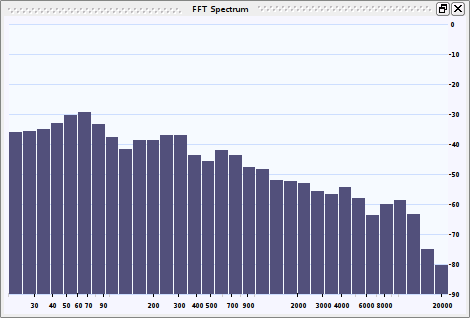
\includegraphics[width=0.6\textwidth]{images/fft1}
	\caption{The FFT spectrum analyzer decomposes the master output signal into its frequencies.}
	\label{fig_fft1}
\end{figure}

The configuration dialog shown in \FigT\ \ref{fig_fft3} allows to define the dB- and frequency range to be displayed. The audible spectrum ranges from 20 to approximately 18000 Hz, whereas CDs range from 20 to 22050 Hz. These are thus recommended values for the lower and upper frequency limit. The upper limit for dB values on the y axis is usually in the range from $-6$ to $+6$ dB, the lower limit between $-60$ and $-120$ dB. The number of bands can be chosen freely, but high numbers ($\geq 128$) cause significantly higher CPU load.

The feature ``show average spectrum'' activates a curve which calculates the average frequency spectrum by accumulating the values as long as Traverso is playing back. The curve is reset if playback is restarted or by the key action \sact{L}. The average curve can also be toggled by the key action \sact{M}, and as soon as there is average data available, the curve can be exported either as raw numbers, or in \texttt{grace} format, which can be opened with the program XmGrace (key action \dact{Return}).

Parameters related to the FFT calculation can be configured in the section ``Advanced Options''. The FFT size determines the lower end of the spectrum; larger FFTs extend to lower frequencies, but cause more CPU load. The lowest frequency captured by the FFT is calculated as:
\[
f_{min} = \frac{\textrm{Samplerate}}{\textrm{FFT size}}
\]
The \emph{lowest} frequency of an FFT of 1024 samples from an audio signal sampled at 44100~Hz is thus 43.1~Hz. Increasing the FFT size to 2048 samples increases the range to 21.5~Hz. The \emph{highest} frequency captured by an FFT is
\[
f_{max} = 0.5 \cdot \textrm{Samplerate}
\]
For audio data sampled at 44100~Hz the upper limit is thus fixed at 22050~Hz.

The windowing function is highly FFT specific and it is beyond the scope of this document to explain it in detail. Users who don't have a particular reason to use a different function are adviced to use the ``Hanning'' window.

\begin{figure}
	\centering
	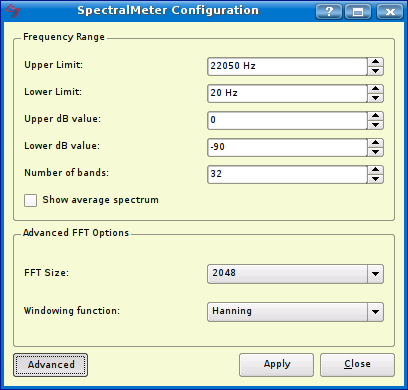
\includegraphics[width=0.7\textwidth]{images/fft3}
	\caption{A configuration dialog called with \sact{E} allows to configure many parameters of the FFT spectrum analyzer.}
	\label{fig_fft3}
\end{figure}

\emph{Note:} For very large FFT sizes the update rate of the spectrum analyzer becomes low. This is not necessarily caused by CPU overload (although CPU load becomes higher for larger FFT sizes), but by the fact that it takes some time to fill the buffers with such large amounts of data. The widget waits until the buffers are full before updating the display.


